\section{HSS approximation of Cauchy-like matrix $C$} 
\label{sec:HSSintro}

While the HODLR format has the advantage of being relatively simple to implement, significant savings in Steps 2 and 3 of Algorithm~\ref{alg:generalsolver} are possible if  more complicated hierarchical low-rank formats, such as the HSS format, are used. 

Compared to HODLR, HSS features additional recursive relations in the off-diagonal low-rank factors across partition levels~\cite{bebendorf2008hierarchical,hackbusch2015hierarchical, martinsson2011fast}. 
Specifically, let \smash{$\widetilde{C}$}  be a HODLR matrix, and let every off-diagonal HODLR block \smash{$\widetilde{C}_v$}
be expressed as \smash{$\widetilde{C}_v = U_v B_{v} V_{\tilde{v}^*}$}, where \smash{$\tilde{v}$} is the sibling vertex of $v$ in the tree $\mathcal T$ determining the HODLR partitioning. For simplicity, we assume that each such block is of equal rank $p$ and, hence, \smash{$B_{v,\tilde v}$} is $p \times p$. 
For an HSS matrix \smash{$\widetilde{C}$}, the left factor \smash{$U_v$} for a parent vertex $v$ admits the expression
\begin{equation} 
\label{eq:HSS_facteveryorU}
U_v = \begin{bmatrix} U_{2v+1} & 0 \\ 0 & U_{2v+2} \end{bmatrix} R_v, \quad R_v \in \mathbb{C}^{2p \times p}.
\end{equation}
In other words, the columns of \smash{$U_v$} are contained in the subspace spanned by the direct sum of the left factors at the children vertices.
The transfer of information from the children to the parent vertex is encoded in the transfer matrix \smash{$R_v$}. If the sibling \smash{$\tilde v$} is a parent vertex, the right factor \smash{$V_{\tilde v}$} also satisfies a similar relation:
\begin{equation} 
\label{eq:HSS_factorV}
V_{\tilde{v}} = \begin{bmatrix} V_{2\tilde v+1} & 0 \\ 0 & V_{2\tilde v+2} \end{bmatrix} W_{\tilde{v}}, \quad W_{\tilde{v}} \in \mathbb{C}^{2p \times p}.
\end{equation}
Expanding the recursions~\eqref{eq:HSS_facteveryorU}--\eqref{eq:HSS_factorV},
the factorization \smash{$\widetilde C_1 = U_1B_{1,2} V_2^* $} for the example from Figure~\ref{fig:HODLRandTree} takes the form
\[
 \underbrace{\begin{bmatrix} 
U_{7} & & & \\
& U_{8} & & \\
& & U_{9} & \\
& & & U_{10}
\end{bmatrix}}_{4 \nmin \times 4 p} \underbrace{\begin{bmatrix} R_3 & \\ & R_4\end{bmatrix}}_{4p \times 2p} \underbrace{R_1}_{2p\times p} \underbrace{B_{1,2}}_{p \times p} W_2^* \begin{bmatrix} W_5^* & \\ & W_6^*\end{bmatrix} \begin{bmatrix} 
V_{11}^* & & & \\
& V_{12}^* & & \\
& & V_{13}^* & \\
& & & V_{14}^*
\end{bmatrix},
\]
where $\nmin$ denotes the minimum block size.

In general, the recursion explained above allows one to store only the small matrices \smash{$R_v$}, \smash{$W_v$}, and \smash{$B_{v,\tilde v}$} for every parent vertex $v\in \mathcal T$. On the lowest level \smash{$\widehat{\ell}$} of the tree $\mathcal T$,
one explicitly stores the $\nmin \times \nmin$ diagonal blocks as well as \smash{$U_v, B_{v,\tilde v},$ and $V_v$}  for each of the \smash{$2^{\widehat{\ell}}$} leaf vertices $v$. We refer to the representation in terms of these small matrices as the \textit{HSS format} of \smash{$\widetilde{C}$}. Storing \smash{$\widetilde{C}$} in the HSS format requires only $\mathcal{O}(n p)$ memory, which is about a factor $\log_2 n$ smaller compared to the HODLR format with HODLR rank $p$.

\subsection{Superfast HSS-based solvers}

\label{sec:advantagesHSS} 

The HSS format not only reduces the cost for storing but also the cost for operating with a matrix $\widetilde{C}$. For example, a matrix-vector product \smash{$\widetilde{C}y$} can be computed in $\mathcal{O}(n p)$ operations~\cite[Alg. 1]{martinsson2011fast}.
Crucially, the HSS format also makes the solution of a linear system \smash{$\widetilde{C}\widetilde{x} = \widetilde{b}$} especially efficient to compute. In the following, we only sketch how such fast solvers work and refer to~\cite{chandrasekaran2006fast,xia2012superfast} for more details. After computing a so-called ULV factorization~\cite{chandrasekaran2006fast} -- a recursive unitary transformation to triangular form that takes advantage of the nested hierarchical structure -- a fast merge-and-backward-substitution routine, followed by a forward-substitution scheme, can be used to solve the linear system. This ULV factorization and the subsequent solution only require \smash{$\mathcal{O}(p^2n)$} and \smash{$\mathcal{O}(p n)$} operations, respectively.  In~\cite{xia2012superfast},  a related ULV-like solver is introduced that relaxes the requirement of  using unitary transformations, saving about a factor of 2 over the standard ULV solver~\cite[Sec.~3.6]{xia2012superfast}. For this approach to work, every \smash{$U_v, V_v, R_v$,} and \smash{$W_v$} in the HSS format need to originate from interpolative decompositions.\footnote{In our experiments in \cref{sec:practicalsolver}, we use the interpolative decompositions described in Section~\ref{sec:int_decomp}, but then orthogonalize and apply the standard ULV solver.}

Our focus in this work is not the reproduction of the HSS solvers already developed in~\cite{chandrasekaran2007superfast, martinsson2011fast, xia2012superfast}. Instead, we develop an fADI-based interpolative decomposition for appropriate HSS blocks. This HSS approximation is cheap and deterministic, and it allows for any HSS solver to be used, even the specialized one in~\cite{xia2012superfast}.

\subsection{HSS rows and columns, HSS rank}
\label{sec:HSSrowscols}


Our construction of an HSS approximation to $C$ proceeds via compressing the so-called HSS rows and columns~\cite{benzi2016matrices, martinsson2011fast,xia2010fast}.
% \sout{In order to understand how well the Cauchy-like matrix $C$ can be approximated by an HSS matrix, we need to introduce the concept of HSS rows and HSS columns. For this purpose, recall that we used \smash{$J_v$} to denote the row indices of an off-diagonal block \smash{$C_v$} for a vertex $v$ in the tree \smash{$\mathcal{T}$} defining the block partition.}
We call
\[
 C_v^{\mathrm{row}} = C(J_v, J_v^c), \quad J_v^c = \{ 0, \ldots, n-1\} \setminus J_v
\]
an HSS row. This selects the block row containing \smash{$C_v$}, but excludes the diagonal block in that row, as shown in Figure~\ref{fig:HSSrows_cols}.
Similarly, an HSS column is defined as \smash{$C_{v}^{\mathrm{col}} = C(J_{v}^c, J_{v})$}.  
As discussed in~\cite{xia2010fast}, the construction of the HSS matrix \smash{$\widetilde{C}$} with each block \smash{$\widetilde{C}_v$} of rank at most $p$ is possible if and only if every HSS row and column of \smash{$\widetilde{C}$} has rank at most $p$. 
This suggests to define the \smash{$(\epsilon, \mathcal{T})$}-HSS rank of $C$  as the smallest $p$ such that \smash{$\erank(C^{\mathrm{row}}_v), \erank(C^{\mathrm{col}}_v) \leq p$} for every $v \in \mathcal{T} \setminus \{0\}$. Applying Theorem~\ref{thm:bounds}
to $( C^{\mathrm{row}}_v )^*$ and
$C^{\mathrm{col}}_v$ with $m \le n/2$ and $\sep = 1$, 
yields the following result.
\begin{lemma} 
\label{lemma:HSS_rank}
For a perfectly balanced binary
tree $\mathcal{T}$, the integer
\[
p = \rho \big\lceil 2\pi^{-2} \log (2n) \log(4 \epsilon^{-1} ) \big\rceil
\]
 is an upper bound on the \smash{$(\epsilon, \mathcal{T})$}-HSS rank of $C$.
\end{lemma}

\begin{figure}
\centering
\begin{tikzpicture}[scale=0.27, every node/.style={scale=0.87}]
%matrix tesselation
\draw[black, thick](0,0)--(8,0);
\draw[black, thick] (0,0)--(0,8);
\draw[black, thick] (8,0)--(8,8);
\draw[black, thick] (0,8)--(8,8);
\draw[black, thick](4,0)--(4,8);
\draw[black, thick](0,4)--(8,4);
\draw[black, thick](2, 4)--(2, 8); 
\draw[black, thick](0, 6)--(4, 6); 
\draw[black, thick](6, 0)--(6, 4); 
\draw[black, thick](4, 2)--(8,2);
\draw[black, thick](0, 7)--(2, 7); 
\draw[black, thick](1,6)--(1,8);
\draw[black, thick](2, 5)--(4,5); 
\draw[black, thick](3, 4)--(3, 6); 
\draw[black, thick](4, 3)--(6,3); 
\draw[black, thick](5,2)--(5, 4); 
\draw[black, thick](6,1)--(8,1); 
\draw[black, thick](7, 0)--(7, 2); 
%fill HSS row 
\draw [pattern=north west lines, pattern color=blue] (0,5) rectangle (2,6);
\draw [pattern=north west lines, pattern color=blue] (3,5) rectangle (8,6);
\draw [pattern=north west lines, pattern color=red] (0,4) rectangle (3,5);
\draw [pattern=north west lines, pattern color=red] (4,4) rectangle (8,5);
%label
\node[] at (4, -1) {(a)}; 
\end{tikzpicture}
\begin{tikzpicture}[scale=0.27, every node/.style={scale=0.87}]
\hspace{10pt}
%matrix tesselation
\draw[black, thick](0,0)--(8,0);
\draw[black, thick] (0,0)--(0,8);
\draw[black, thick] (8,0)--(8,8);
\draw[black, thick] (0,8)--(8,8);
\draw[black, thick](4,0)--(4,8);
\draw[black, thick](0,4)--(8,4);
\draw[black, thick](2, 4)--(2, 8); 
\draw[black, thick](0, 6)--(4, 6); 
\draw[black, thick](6, 0)--(6, 4); 
\draw[black, thick](4, 2)--(8,2);
\draw[black, thick](0, 7)--(2, 7); 
\draw[black, thick](1,6)--(1,8);
\draw[black, thick](2, 5)--(4,5); 
\draw[black, thick](3, 4)--(3, 6); 
\draw[black, thick](4, 3)--(6,3); 
\draw[black, thick](5,2)--(5, 4); 
\draw[black, thick](6,1)--(8,1); 
\draw[black, thick](7, 0)--(7, 2); 
%fill HSS row 
\draw [pattern=north west lines, pattern color=purple] (0,4) rectangle (2,6);
\draw [pattern=north west lines, pattern color=purple] (4,4) rectangle (8,6);
%label
\node[] at (4, -1) {(b)}; 
\end{tikzpicture}
\begin{tikzpicture}[scale=0.27, every node/.style={scale=0.87}]
\hspace{20pt}
%matrix tesselation
\draw[black, thick](0,0)--(8,0);
\draw[black, thick] (0,0)--(0,8);
\draw[black, thick] (8,0)--(8,8);
\draw[black, thick] (0,8)--(8,8);
\draw[black, thick](4,0)--(4,8);
\draw[black, thick](0,4)--(8,4);
\draw[black, thick](2, 4)--(2, 8); 
\draw[black, thick](0, 6)--(4, 6); 
\draw[black, thick](6, 0)--(6, 4); 
\draw[black, thick](4, 2)--(8,2);
\draw[black, thick](0, 7)--(2, 7); 
\draw[black, thick](1,6)--(1,8);
\draw[black, thick](2, 5)--(4,5); 
\draw[black, thick](3, 4)--(3, 6); 
\draw[black, thick](4, 3)--(6,3); 
\draw[black, thick](5,2)--(5, 4); 
\draw[black, thick](6,1)--(8,1); 
\draw[black, thick](7, 0)--(7, 2); 
%fill HSS row 
\draw [pattern=north west lines, pattern color=blue] (4,0) rectangle (6,2);
\draw [pattern=north west lines, pattern color=blue] (4,4) rectangle (6,8);
\draw [pattern=north west lines, pattern color=red] (6,2) rectangle (8,8);
%label
\node[] at (4, -1) {(c)}; 
\end{tikzpicture}
\begin{tikzpicture}[scale=0.27, every node/.style={scale=0.87}]
\hspace{30pt}
%matrix tesselation
\draw[black, thick](0,0)--(8,0);
\draw[black, thick] (0,0)--(0,8);
\draw[black, thick] (8,0)--(8,8);
\draw[black, thick] (0,8)--(8,8);
\draw[black, thick](4,0)--(4,8);
\draw[black, thick](0,4)--(8,4);
\draw[black, thick](2, 4)--(2, 8); 
\draw[black, thick](0, 6)--(4, 6); 
\draw[black, thick](6, 0)--(6, 4); 
\draw[black, thick](4, 2)--(8,2);
\draw[black, thick](0, 7)--(2, 7); 
\draw[black, thick](1,6)--(1,8);
\draw[black, thick](2, 5)--(4,5); 
\draw[black, thick](3, 4)--(3, 6); 
\draw[black, thick](4, 3)--(6,3); 
\draw[black, thick](5,2)--(5, 4); 
\draw[black, thick](6,1)--(8,1); 
\draw[black, thick](7, 0)--(7, 2); 
%fill HSS row 
\draw [pattern=north west lines, pattern color=purple] (4,4) rectangle (8,8);
%label
\node[] at (4, -1) {(d)}; 
\end{tikzpicture}
\caption{Various HSS rows and columns for a tree of depth $3$ (see Figure~\ref{fig:HODLRandTree}). In (a), the two HSS rows $C_9^{\mathrm{row}}$(blue) and $C_{10}^{\mathrm{row}}$ (red) are shown.  These are the children of the row $C_4^{\mathrm{row}}$, shown in (b). The two HSS columns $C_5^{\mathrm{col}}$ (red)  and $C_6^{\mathrm{col}}$ (blue)  in (c) are the children of the parent $C_2^{\mathrm{col}}$ in (d). }
\label{fig:HSSrows_cols}
\end{figure}


\subsection{Approximation by interpolative decompositions} 
\label{sec:int_decomp}

By~\cite[Thm. 4.7]{KMR2019}, there is an HSS matrix
$\widetilde C$ of HSS rank $p$, with the value of $p$ stated in Lemma~\ref{lemma:HSS_rank}, such that
$\|C- \widetilde C\|_2 \lesssim \sqrt{n} \epsilon$. Standard algorithms~\cite{xia2010fast} for constructing such a compression $\widetilde C$ proceed by recursively compressing the HSS blocks and rows in a bottom-up fashion. The compression on the upper levels by orthogonal projections is expensive, requiring already $\mathcal O(n^2)$ operations for just evaluating the entries of the corresponding HSS block columns/rows. Interpolative decompositions~\cite{cheng2005compression,martinsson2011fast, xia2012superfast} are a common approach to mitigate this problem. In this section, we explain how interpolative decompositions can be combined with fADI to cheaply construct HSS approximations to $C$.

\subsubsection{Interpolative decompositions on the leaf level}  \label{sec:leafinterpolation}

%We now discuss how to construct an approximate HSS factorization of $C$ using a fADI-based interpolative decomposition to approximate each HSS row and column.  
%A standard approach  involves the use of interpolative decompositions. We first describe how to construct such approximations at the leaf level. %Once the leaf interpolative decompositions are known, standard strategies can be applied to move upward along $\mathcal{T}$ and derive the requisite factors for the HSS approximation. We refer to~\cite{} for a detailed description of the so-called merge process.  
%and then discuss how to use the leaf factorizations to move up $\mathcal{T}$ and find the requisite factors.
%~\cite{martinsson2011fast, xia2012superfast}
%The structure of interpolative decompositions also allows one to apply the accelerated ULV-like solver from~\cite[Sec.~3.4]{xia2012superfast} in Step 3 of Algorithm~\ref{alg:generalsolver} if desired.
%We briefly review the general use of interpolative decompositions in forming HSS factorizations. Then, in section~\ref{sec:HSSfadi}, we describe how our bounds and fADI can be used to construct specific, displacement-based  interpolative decompositions.

Consider a leaf $v \in \mathcal T$ with sibling $\tilde v$. We aim at constructing 
a two-sided interpolative decomposition~\cite{cheng2005compression} for the corresponding off-diagonal block $C_v \in \C^{m \times m}$, $m = \nmin$, of the form
\begin{equation}
\label{eq:block_factors}
 C_v \approx \widetilde{C}_v = U_v B_{v, \tilde{v}} V_{\tilde{v}}^*, \quad B_{v, \tilde{v}} = C(\mathbb{J}_v, \mathbb{K}_{\tilde{v}}),
 \end{equation} 
where \smash{$\mathbb J_v \subset J_v$} and \smash{$\mathbb K_{\tilde{v}} \subset J_{\tilde{v}}$} are index subsets, each of cardinality $p \ll m$. This decomposition is obtained from constructing one-sided 
interpolative decompositions for the corresponding HSS block row/column:
\begin{equation} 
\label{eq:HSSrowinterp2} 
C_v^{\mathrm{row}} \approx \widetilde{C}_v^{\mathrm{row}}  = U_v  C_v^{\mathrm{row}}(\mathbb{J}_v, \, :\,), \quad 
C_{\tilde v}^{\mathrm{col}} \approx \widetilde{C}_{\tilde v}^{\mathrm{col}}  = C_{\tilde v}^{\mathrm{col}}(\, :\,, \mathbb K_{\tilde v}) V_{\tilde v}^*.
\end{equation}
This requires that the selected subset $\mathbb{J}_v$ of rows represents a good approximation 
to the row space of $C_v^{\mathrm{row}}$
and, analogously, that the 
selected subset $\mathbb{K}_{\tilde v}$ of columns represents a good approximation 
to column space of $C_{\tilde v}^{\mathrm{col}}$. Both are instances of the column subset selection problem~\cite{broadbent2010subset}, for which numerous algorithms have been developed, including 
the column-pivoted QR (CPQR)~\cite{GolubVanLoan2013}, (strong) rank-revealing QR decomposition~\cite{gu1996efficient} or Osinsky's algorithm~\cite{Osinsky2023}.
However, applying such algorithms directly to HSS block rows/columns is expensive. For example, \smash{$C_v^{\mathrm{col}}$} is of size \hbox{$(n\!-\!m) \times m$}, so the cost depends at least linearly on the ``long" dimension $n$.  One can do better with carefully implemented randomized methods~\cite{martinsson2011fast,xia2012superfast}, but even this approach requires an initial precomputation that multiplies the uncompressed matrix $C$ with an $n \times \Theta(p)$ Gaussian random matrix.\footnote{In~\cite{xia2012superfast}, this step is greatly improved with a fast matrix-vector multiplication routine for $C$ based on its relationship to the Toeplitz matrix $T$.} 
In the following, we show how the interpolative decompositions~\eqref{eq:HSSrowinterp2} 
can be found deterministically using fADI with a cost that depends only on $m$ and $p$.

We focus on the selection of $\mathbb{J}_v$; the process for finding $\mathbb{K}_{\tilde v}$ is entirely analogous.
Set \smash{$X := C_v^{\mathrm{row}}$}.
We know from~\eqref{eq:cauchylike-disp} that $X$ satisfies \[
D_JX - XD_K = \widetilde G_J \widetilde H_K^*, \quad J = J_v, \quad K = J_v^{c}.
\]
After $k$ iterations of fADI, the approximation \begin{equation}\label{eq:adi2}
X \approx X^{(k)} = ZW^*, \quad  Z  \in \mathbb{C}^{m \times p }, \quad p = k \rho,
                                                \end{equation}
is constructed. To find an approximate one-sided row interpolative decomposition, the (large) matrix $W$ is actually not needed. A key advantage of fADI is that it constructs $Z$ independently from $W$ using only the $m \times \rho$ matrix \smash{$\widetilde G_J$} and the $m \times m$ diagonal matrix \smash{$D_J$} (see \cref{alg:fadicauchy}). In turn, the construction of $Z$ only requires $\mathcal{O}(m \rho)$ operations.


One continues from~\eqref{eq:adi2} by selecting a good subset of rows in the (smaller) factor $Z$. For convenience, 
our numerical experiments apply CPQR to $Z^*$ for this purpose. This has a computational cost of only \smash{$\mathcal{O}(m p^2)$} operations and is usually a safe choice.\footnote{Despite famous adversarial examples where CPQR fails, it is considered highly reliable in practice~\cite{gu1996efficient}.} Better theoretical bounds are obtained, at the same asymptotic cost, by using more sophisticated methods, such as Osinsky's algorithm~\cite{Osinsky2023}; see also~\cite{Cortinovis2024}. For this purpose, we first compute a QR decomposition $Z = QR$ with $Q \in \C^{m\times p}$. Applying Algorithm 2 from~\cite{Osinsky2023} to $Q^*$ returns an index set
$\mathbb I_v$ of cardinality $p$ such that
\begin{equation} \label{eq:osinsky}
 \|Z \cdot Z(\mathbb I_v,:)^{-1} \|_2 = 
 \|Q \cdot Q(\mathbb I_v,:)^{-1} \|_2 \le \sqrt{1+p(m-p)};
\end{equation}
see~\cite[Thm. 5]{Osinsky2023}. Setting $U_v = Z \cdot Z(I_v,:)^{-1}$ concludes the construction of the desired
approximation $C_v^{\mathrm{row}} \approx U_v  C_v^{\mathrm{row}}({J}_v, \, :\,)$.

\begin{lemma} 
\label{lemma:int_decomp_error_leaf}
Set $X = C_v^{\mathrm{row}} \in \C^{m \times (n-m)}$.
The approximation $X \approx U_v X(\mathbb{J}_v, \, : \,)$ described above satisfies the error bound
\begin{equation} 
\label{eq:HSS_fadi_error}
\|X - U_v X(\mathbb{J}_v, \, : \,)\|_2 \leq 4 \xi^{-k} \big( 1 + \sqrt{1+p(m-p)}\big) \|X\|_2,
\end{equation}
with \smash{$\xi = \exp(  \pi^2 / ( 2 \log( 4 m  ) )$} and $p = k \rho$.
\end{lemma}
\begin{proof}
Observe that
$$ \|X - U_v X(\mathbb{J}_v, \, : \,)\|_2 \leq  \|X - ZW^*\|_2 + \|ZW^* - X(\mathbb{J}_v, \, : \,)\|_2.$$
The second term is bounded by
\[
 \|ZW^* - U_v X(\mathbb{J}_v, \, : \,)\|_2
 = \big\|
 U_v \big(
 Z(\mathbb J_v,:) W^* X(\mathbb{J}_v, \, : \,)
 \big) 
 \big\|_2 \le \|U_v\|_2\|  ZW^* - X  \|_2.
\]
The proof is concluded by using~\eqref{eq:osinsky} for bounding $\|U_v\|_2$, and $\|X - ZW^*\|_2 \leq 4 \xi^{-k} \|X\|_2$,
which follows from a straightforward extension of~\cref{corr:ADIbounds}.
\end{proof}


We view~\eqref{eq:HSS_fadi_error} as the deterministic analogue to the error bounds supplied in~\cite[Eq.~3.6]{xia2012superfast} for interpolative decompositions based on randomized linear algebra. There, one finds  \smash{$ \Theta_v X(\mathbb J_v, \; : \;)$}, which is a rank $p + \mu$ approximate row interpolative decomposition for $X$, with $\mu$ selected as a small  oversampling parameter~\cite{halko2011finding}. Properties of Gaussian random matrices can be used to show that with probability \smash{$1 - 6 \mu^{-\mu}$}, the error is bounded as~\cite[Eq.~(3.6)]{xia2012superfast} 
\begin{equation} 
\label{eq:Rand_err}
\|X - \Theta_v X(\mathbb J_v, \; : \;)\|_2 \leq \big( 1 + 11 \sqrt{m(p + \mu)}\big) \sigma_{p+1}(X). 
\end{equation}
Using~\eqref{eq:bound_zolo_arcs} and~\eqref{eq:zolobound_svs}, our bounds show that \smash{$\sigma_{p+1}(X) \leq  4 \xi^{-\lfloor p/\rho \rfloor } \| X\|_2$}, where $\xi$ is given in~\eqref{eq:bound_zolo_arcs}. This makes~\eqref{eq:Rand_err} explicit so that if one prefers to use a solver based on randomized linear algebra, $p$ can be chosen a priori in order to ensure (w.h.p.) that the relative error is bounded by $\epsilon$. 


\subsection{HSS approximation by recursive interpolative decomposition}
\label{sec:merge}

Once the interpolative decomposition~\eqref{eq:block_factors} is known for each block on the finest level \smash{$\widehat{\ell}$} of \smash{$\mathcal{T}$}, the remaining factors associated with the non-leaf vertices of \smash{$\mathcal{T}$} are determined
in a bottom-up fashion. We briefly describe the process of merging from the leaf level up to the next coarsest level, but refer to~\cite{wilber2021computing} for substantial details on such processes, which are admittedly technical but also standard and well-established.

Let $v$ be a vertex on level \smash{$\ell = \widehat{\ell}\! -\! 1$}. Then, as before, we aim at finding an approximation \smash{$C_v \approx \widetilde{C}_v = U_vB_{v, \tilde{v}}V_{\tilde{v}}^*$}. It is assumed that the outer factor  \smash{$U_v$} and \smash{$V_{\tilde{v}}$} satisfy the relations~\eqref{eq:HSS_facteveryorU} and~\eqref{eq:HSS_factorV}, respectively, and it thus only remains to determine \smash{$R_v$}, \smash{$W_{\tilde{v}}$}, and the index sets $\mathbb J_v$, $\mathbb K_{\tilde{v}}$ defining \smash{$B_{v, \tilde{v}} = C(\mathbb J_v, \mathbb K_{\tilde{v}})$}.  Consider the associated HSS row \smash{$C_v^{\mathrm{row}}$}. Its children HSS rows \smash{$C_{2v+1}^{\mathrm{row}}$, $C_{2v+2}^{\mathrm{row}}$} are approximated by the algorithm discussed in Section~\ref{sec:leafinterpolation}:
$$C_{2v+j}^{\mathrm{row}}(\, : \, , \, J_v^c) \approx U_{2 v+j} C_{2v+j}^{\mathrm{row}}(\mathbb{J}_{2v+j}, \, J_v^c\,).$$ Using these decompositions, we can write
\begin{equation} 
\label{eq:non_leaf_row}
 C_v^{\mathrm{row}} \approx \begin{bmatrix} U_{2v+1} & 0 \\ 0 & U_{2v+2} \end{bmatrix} C_v(\widehat{\mathbb J}, \, : \,),
 \end{equation} 
where \smash{$\widehat{\mathbb J}$} is the index set with respect to the block \smash{$C_v^{\mathrm{row}}$} that selects the $2p$ rows indexed by \smash{$\mathbb{J}_{2v+1} \cup \mathbb{J}_{2v+2}$}; see~\cref{fig:basis_rows}~(b).  

With the cascading factors in~\eqref{eq:HSS_facteveryorU} in mind, we simply apply the fADI-based row interpolative decomposition from Section~\ref{sec:leafinterpolation} to the submatrix $C_v(\widehat{\mathbb J},:)$.  Theorem~\ref{thm:bounds} and Lemma~\ref{lemma:int_decomp_error_leaf} hold for this submatrix, which is also Cauchy-like and therefore has a useful displacement structure. 
This process chooses a size-$p$ subset $\mathbb J_v$ of the $2 p$ rows comprising \smash{$C_v(\widehat{\mathbb{J}}, \, : \,)$}; see \cref{fig:basis_rows}~(c), and it also produces $R_v$.  An analogous method is applied to \smash{$C_{\tilde{v}}^{\mathrm{col}}$} to find \smash{$\mathbb K_{\tilde{v}}$} and \smash{$W_{\tilde{v}}$}. This procedure can be repeated at each level as we traverse \smash{$\mathcal{T}$} from the bottom to the top in order to produce an approximate HSS factorization of the entire matrix $C$~\cite{martinsson2011fast}. 

\begin{figure}
\centering
\label{fig:basis_rows}
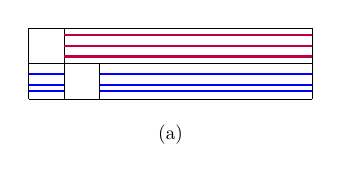
\begin{tikzpicture}[scale=0.45, every node/.style={scale=0.7}]
%matrix tesselation
\draw[black](0,0)--(0,2);
\draw[black] (0,0)--(8,0);
\draw[black] (0,2)--(8,2);
\draw[black] (8,0)--(8,2);
\draw[black] (2,0)--(2,1);
\draw[black] (0,1)--(8,1);
\draw[black] (1,0)--(1,2);
%\draw[black, thick] (4,0)--(4,2);
\draw[purple, thick](1, 1.5)--(8, 1.5); 
\draw[purple, thick](1, 1.2)--(8, 1.2); 
\draw[purple, thick](1, 1.8)--(8, 1.8); 
\draw[blue, thick](2, .4)--(8, .4); 
\draw[blue, thick](2, .23)--(8, .23); 
\draw[blue, thick](2, .7)--(8, .7);  
\draw[blue, thick](0, .4)--(1, .4); 
\draw[blue, thick](0, .23)--(1, .23); 
\draw[blue, thick](0, .7)--(1, .7);  
\node[] at (4, -1) {(a)}; 
\end{tikzpicture}
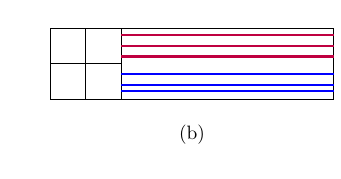
\begin{tikzpicture}[scale=0.45, every node/.style={scale=0.7}]

\hspace{8pt} 

\draw[black](0,0)--(0,2);
\draw[black] (0,0)--(8,0);
\draw[black] (0,2)--(8,2);
\draw[black] (8,0)--(8,2);
\draw[black] (2,0)--(2,2);
\draw[black] (0,1)--(2,1);
\draw[black] (1,0)--(1,2);
%\draw[black, thick] (4,0)--(4,2);
\draw[purple, thick](2, 1.5)--(8, 1.5); 
\draw[purple, thick](2, 1.2)--(8, 1.2); 
\draw[purple, thick](2, 1.8)--(8, 1.8); 
\draw[blue, thick](2, .4)--(8, .4); 
\draw[blue, thick](2, .23)--(8, .23); 
\draw[blue, thick](2, .7)--(8, .7);  
%\draw[blue, thick](0, .4)--(1, .4); 
%\draw[blue, thick](0, .23)--(1, .23); 
%\draw[blue, thick](0, .7)--(1, .7);  
\node[] at (4, -1) {(b)}; 
\end{tikzpicture}
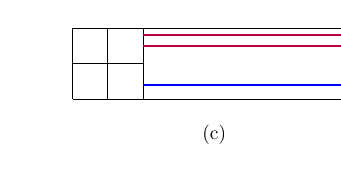
\begin{tikzpicture}[scale=0.45, every node/.style={scale=0.7}]

\hspace{16pt}

\draw[black](0,0)--(0,2);
\draw[black] (0,0)--(8,0);
\draw[black] (0,2)--(8,2);
\draw[black] (8,0)--(8,2);
\draw[black] (2,0)--(2,2);
\draw[black] (0,1)--(2,1);
\draw[black] (1,0)--(1,2);
%\draw[black, thick] (4,0)--(4,2);
\draw[purple, thick](2, 1.5)--(8, 1.5); 
\draw[purple, thick](2, 1.8)--(8, 1.8); 
\draw[blue, thick](2, .4)--(8, .4); 
%\draw[blue, thick](2, .23)--(8, .23);
\node[] at (4, -1) {(c)}; 
\end{tikzpicture}
\caption{ (a) Selected row vectors indexed by \smash{$\mathbb{J}_{2v+j}$} for the two HSS rows \smash{$C_{2v+j}^{\mathrm{row}} \approx U_{2v+j} C_{2v+j}^{\mathrm{row}}(\mathbb{J}_{2v+j}, \, : \,)$},  $j = 1$ (red) and $j = 2$ (blue).  (b) The HSS row \smash{$C_v^{\mathrm{row}}$} is over-resolved by~\eqref{eq:non_leaf_row}, a row interpolative decomposition with  basis vectors taken as the union of the subsampled basis vectors (colored lines) of the children rows.  At this coarser level, we re-apply  interpolative decomposition to the submatrix of \smash{$C_v^{\mathrm{row}}$} consisting only of the colored basis row vectors in (b). This compresses the representation  by choosing a subselection of the colored row vectors as a new, reduced basis approximately spanning the row space of \smash{$C_v^{\mathrm{row}}$}, as shown in (c).}
\end{figure}


\subsection{A faster HSS factorization scheme}
\label{sec:cauchyhadamard}
As with the HODLR approximation to $C$, the identity~\eqref{eq:cauchydisp} can be used to improve the overall cost of the HSS factorization.  We take advantage of this when performing fADI on the lowest level $\hat \ell$ of the partitioning determined by $\mathcal T$. It suffices to find fADI approximants only for the first HSS row and column of $\mathscr{C}$.  Then, we use these approximations and~\eqref{eq:hadamard_off} to cheaply compute the left factors of the low-rank approximations for every level-$\hat \ell$ HSS row and column of $C$. Once this is done, CPQR or Osinsky's algorithm are used find interpolative decompositions from each of these low rank approximations. 

In principle, one could go further with this idea, and cheaply compute interpolative decompositions \smash{$\mathscr{C}_v = \mathcal{U}_v \mathscr{C}(J_v, K_{\tilde{v}}) \mathcal{V}_{\tilde{v}}^*$} on every partition level. When the structure of $\mathscr{C}$ is fully exploited and approximations to the submatrices of $C$ are stored in the factored form shown as in~\eqref{eq:eq:hadamard_adi}, the cost for finding an approximate HSS factorization only requires \smash{$\mathcal{O}(\rho^3 \log^3 n \log^3 1/\epsilon)$} operations, that is, this step only depends poly-logarithmically (and not even linearly) on $n$.  This is an effective format for some operations (e.g., matrix-vector products). For solving linear systems,~\eqref{eq:hadamard_off} must be used to assemble low rank approximations to each \smash{$C_v$}. A similar idea is discussed in~\cite{chandrasekaran2007superfast, xia2012superfast}. We note that applying~\eqref{eq:hadamard_off} destroys the interpolative structure of the HSS factors, ruling out the use of the accelerated ULV-like solver from~\cite{xia2012superfast} in Step 3 of Algorithm~\ref{alg:generalsolver}.

\section{A fast HSS-based solver} \label{sec:practicalsolver}

Without exploiting~\eqref{eq:hadamard_adi}, the computational complexity of constructing an HSS approximation to $C$ with our fADI-based interpolative decomposition scheme requires $\mathcal{O}(n (\rho \log n \log 1/\epsilon )^2 )$ operations; a more detailed complexity
analysis can be found in~\cite[Ch.~4]{wilber2021computing}. Putting this together with existing HSS-based solvers for linear systems, the overall complexity for solving $Tx = b$ via \cref{alg:generalsolver} is also $\mathcal{O}(n (\rho \log n \log 1/\epsilon )^2 )$. 

We remark that the bounds in \cref{thm:bounds} indicate that a solver for $Tx=b$ with linear asymptotic complexity in $n$ appears to be possible. This is because submatrices of $C$ sufficiently separated from the main diagonal have $\epsilon$-ranks that are constant with respect to $n$. An appropriate hierarchical matrix approximation with strong admissibility could exploit this fact. Linear inversion routines for such matrices are available~\cite{ambikasaran2014inverse, minden2017recursive}, but the analysis and implementation of these methods are beyond the scope of this paper.


 
 
 %In Figure~\ref{fig:timingsHSS}, we compare the practical performance of the two methods.\footnote{Our implementation includes a few additional cost-saving measures not reflected in the above complexity analysis (see section~\ref{sec:implementation}). Both methods were implemented in MATLAB and timings were performed on \textcolor{red}{computer details here}.} 


 %ULV solver in~\cite{chandrasekaran2006fast}, which is what we use, can still be used if this  The authors of~\cite{xia2012superfast} suggest a re-interpolation strategy that regains the interpolative structure, but such a scheme is not always advantageous over working with $C$ directly. 
